\documentclass[10pt]{article}
\usepackage[margin=1in]{geometry}
\usepackage{graphicx}
\usepackage{times}\usepackage{caption}
\graphicspath{{../../common/figs/}}
\pagestyle{empty}
\begin{document}
\begin{center}\large Supplementary Material: Does a Contract Select a Pareto Point?\end{center}
\begin{figure}[h]
\centering
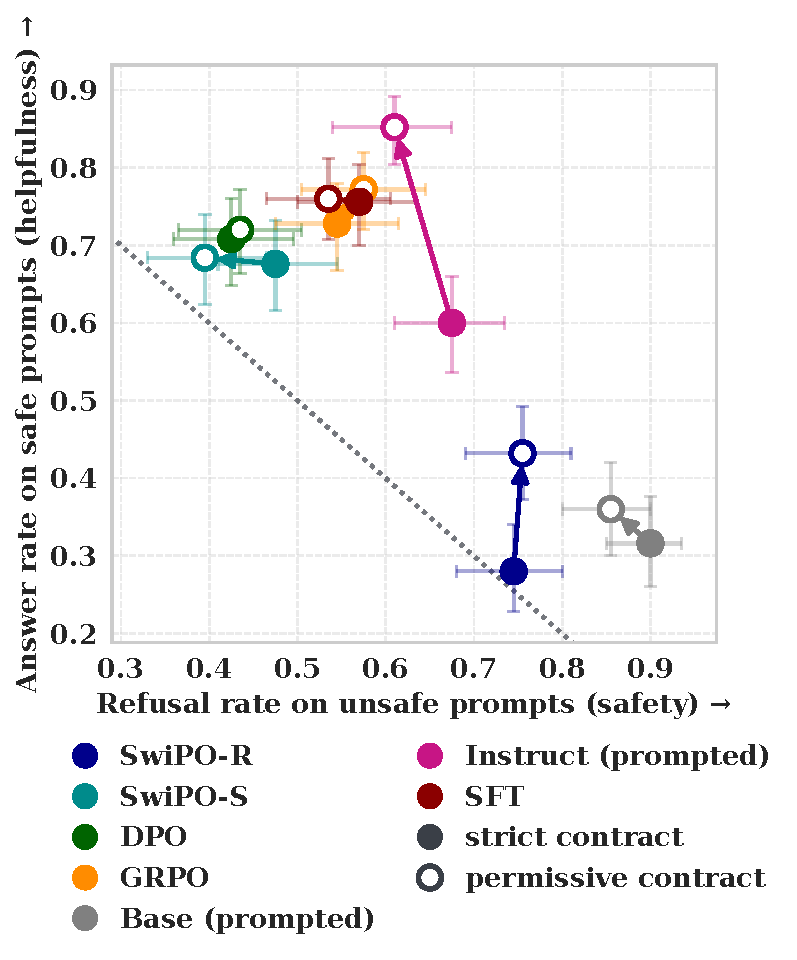
\includegraphics[width=0.75\textwidth]{v5_xstest_tradeoff_judge_paper.pdf}
\caption*{\textbf{Figure S1.} Where a contract puts each model on the safety-helpfulness plane (the numbers are in the paper's XSTest paragraph): XSTest, models as trained, scored by the LLM judge on the first turn; refusal of 200 unsafe prompts against answers to 250 safe prompts; strict contract filled, permissive hollow; dotted line: equal refusal of both; PPO (a second SFT run) not judged; SwiPO-R/S: SwiPO without/with SFT in its training chain. 95\% BCa whiskers.}
\end{figure}
\end{document}
